\documentclass[11pt, a4paper]{article}

\usepackage{amsmath, amssymb, titling}
\usepackage[margin=2.5cm]{geometry}
\usepackage[colorlinks=true, linkcolor=black, urlcolor=black, citecolor=black]{hyperref}
\usepackage{graphicx}
\usepackage{caption}
\usepackage{subcaption}
\usepackage{float}
\usepackage{multicol}
\usepackage{cancel}
\usepackage{fancyhdr, lastpage}
\usepackage{fourier-orns}
\usepackage{xcolor}
\usepackage{nomencl}
\makenomenclature
\usepackage{etoolbox}
\usepackage{sidecap}
\usepackage{adjustbox}
\usepackage{listings}
\usepackage{matlab-prettifier}
\usepackage[T1]{fontenc}

\sidecaptionvpos{figure}{c}
\setlength{\headheight}{18.2pt}
\setlength{\nomlabelwidth}{1.5cm}

% \renewcommand\maketitlehooka{\null\mbox{}\vfill}
% \renewcommand\maketitlehookd{\vfill\null}

\renewcommand{\headrule}{\vspace{-5pt}\hrulefill\raisebox{-2.1pt}{\quad\leafleft\decoone\leafright\quad}\hrulefill}
\newcommand{\parder}[2]{\frac{\partial {#1}}{\partial {#2}}}
% \renewcommand\nomgroup[1]{%
%   \item[\bfseries
%   \ifstrequal{#1}{F}{Far--Away Properties}{%
%   \ifstrequal{#1}{N}{Dimensionless Numbers}{%
%   \ifstrequal{#1}{M}{Matrices}{%
%   \ifstrequal{#1}{D}{Diagonals}{%
%   \ifstrequal{#1}{V}{Vectors}{%
%   \ifstrequal{#1}{P}{Dimensionless Average Properties}{}}}}}}
% ]}

\title{Numerical Methods in Aeronautical Engineering \\ HW3}
\author{Almog Dobrescu ID 214254252}

% \pagestyle{fancy}
\cfoot{Page \thepage\ of \pageref{LastPage}}

\begin{document}

\thispagestyle{empty}
\begin{figure}[H]
    \centering
    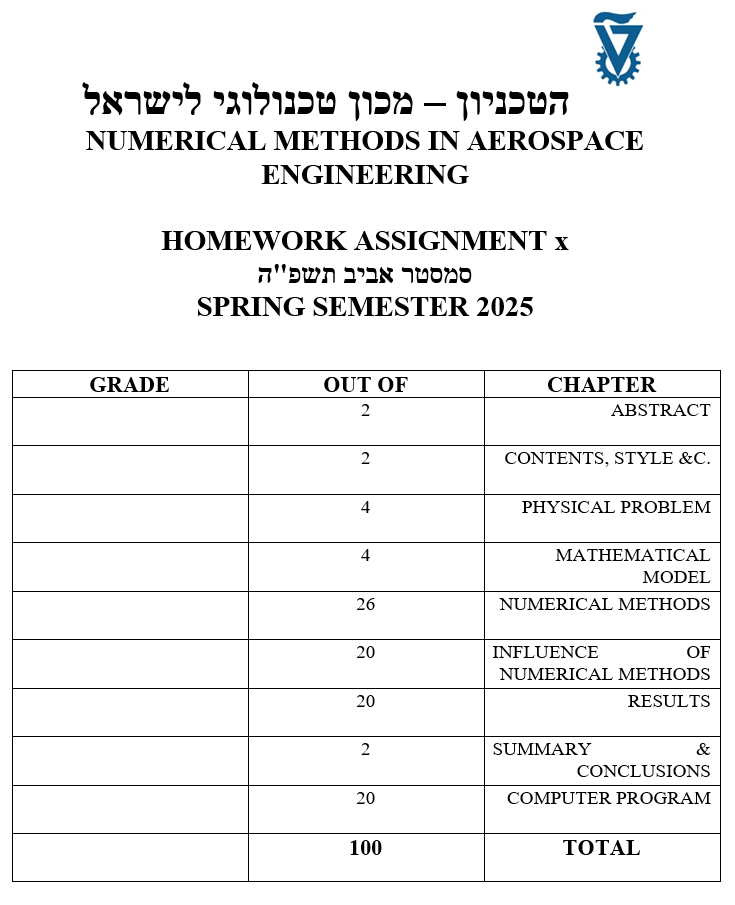
\includegraphics[width=\textwidth]{./../../Cover page for computational assignments 2025.png}
    \label{fig: cover page}
\end{figure}
% \maketitle
\begin{center}
    \Huge
    Almog Dobrescu \qquad ID 214254252 \\ \vspace{0.5cm}
    \today
\end{center}
\newpage

\pagenumbering{roman}
% \setcounter{page}{1}
\begin{abstract}
    hii
\end{abstract}

\tableofcontents
\vfil
\listoffigures
\vfil
\lstlistoflistings
\newpage

\printnomenclature
\newpage

\pagestyle{fancy}
\pagenumbering{arabic}
\setcounter{page}{1}

\section{The Physical Problem}
An incompressible viscose Newtonian fluid flows in a channel.
\begin{figure}[H]
    \centering
    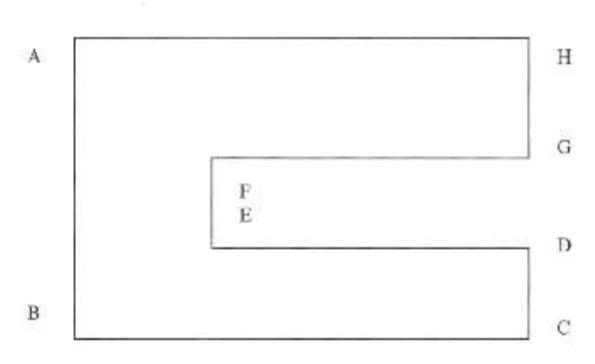
\includegraphics[width=0.7\textwidth]{images/The channel.png}
    \caption{The Channel}
    \label{fig: The Channel}
\end{figure}
Where:
\begin{multicols}{2}
    \begin{itemize}
        \item $AB=12\left[in\right]$
        \item $BC=12\left[in\right]$
        \item $CD=2\left[in\right]$
        \item $DE=6\left[in\right]$
        \item $EF=6\left[in\right]$
        \item $FG=6\left[in\right]$
        \item $GH=4\left[in\right]$
        \item $HA=12\left[in\right]$
    \end{itemize}
\end{multicols}
\noindent The \emph{x}-axis will be from left to right and the \emph{y}-axis will be from bottom to top such that the origin is at point \emph{B}.

\section{The Mathematical Model}
The steady-state velocity of the fluid is given by:
\begin{equation}
    \parder{^2\phi}{x^2}+\parder{^2\phi}{y^2}=-\frac{c}{\mu}
    \nomenclature{$c$}{pressure gradient on the flow in a section}
    \nomenclature{$\mu$}{viscosity of the fluid}
\end{equation}
In our case:
\begin{itemize}
    \item $c=0.0002\left[\frac{lb}{in^3}\right]$
    \item $\mu=0.25\cdot10^{-5}\left[\frac{lb\cdot sec}{in^2}\right]$
\end{itemize}
\subsection{Boundary Conditions}
Since the flow is viscose, the boundary conditions are no penetration and no slip. The flow is at a steady state so the only direction of the flow is normal the sectional area (outside the paper). Hence the velocity at the boundaries is:
\begin{equation}
    \left.\phi\right|_{AB}=\left.\phi\right|_{BC}=\left.\phi\right|_{CD}=\left.\phi\right|_{DE}=\left.\phi\right|_{EF}=\left.\phi\right|_{FG}=\left.\phi\right|_{GH}=\left.\phi\right|_{HA}=0
\end{equation}

\section{The Numerical Methods}
\subsection{Finite Differencing}
In order to solve the partial differential equation we will use finite differences. For the second derivative in space, we will use central differencing:
\begin{equation}
    \begin{array}{c}
        \displaystyle\frac{\phi_{i-1,j}-2\phi_{i,j}+\phi_{i+1,j}}{\Delta x^2}+\mathcal{O}\left(\Delta x^2\right)+\frac{\phi_{i,j-1}-2\phi_{i,j}+\phi_{i,j+1}}{\Delta y^2}+\mathcal{O}\left(\Delta y^2\right)=-\frac{c}{\mu} \\\\
        \displaystyle\left(\phi_{i-1,j}-2\phi_{i,j}+\phi_{i+1,j}\right)\Delta y^2+\left(\phi_{i,j-1}-2\phi_{i,j}+\phi_{i,j+1}\right)\Delta x^2=-\Delta x^2\Delta y^2\frac{c}{\mu}+\mathcal{O}\left(\Delta x^2,\Delta y^2\right) \\\\
        \displaystyle-2\phi_{i,j}\left(\Delta y^2+\Delta x^2\right)+\left(\phi_{i-1,j}+\phi_{i+1,j}\right)\Delta y^2+\left(\phi_{i,j-1}+\phi_{i,j+1}\right)\Delta x^2=-\Delta x^2\Delta y^2\frac{c}{\mu} \\\\
        \displaystyle2\phi_{i,j}\left(\Delta y^2+\Delta x^2\right)=\left(\phi_{i-1,j}+\phi_{i+1,j}\right)\Delta y^2+\left(\phi_{i,j-1}+\phi_{i,j+1}\right)\Delta x^2+\Delta x^2\Delta y^2\frac{c}{\mu} \\\\
        \displaystyle2\phi_{i,j}=\left(\phi_{i-1,j}+\phi_{i+1,j}\right)\frac{\Delta y^2}{\Delta y^2+\Delta x^2}+\left(\phi_{i,j-1}+\phi_{i,j+1}\right)\frac{\Delta x^2}{\Delta y^2+\Delta x^2}+\frac{\Delta x^2\Delta y^2}{\Delta y^2+\Delta x^2}\frac{c}{\mu} \\\\
        \displaystyle\phi_{i,j}=\frac{1}{2}\left(\left(\phi_{i-1,j}+\phi_{i+1,j}\right)\frac{\Delta y^2}{\Delta y^2+\Delta x^2}+\left(\phi_{i,j-1}+\phi_{i,j+1}\right)\frac{\Delta x^2}{\Delta y^2+\Delta x^2}+\frac{\Delta x^2\Delta y^2}{\Delta y^2+\Delta x^2}\frac{c}{\mu}\right)
    \end{array}
    \nomenclature{$i$}{index in the x coordinate}
    \nomenclature{$j$}{index in the y coordinate}
    \nomenclature{$\Delta x$}{step size in the x coordinate}
    \nomenclature{$\Delta y$}{step size in the y coordinate}
\end{equation}
Where:
\begin{itemize}
    \item $\displaystyle\Delta x=\frac{x_{max}-x_{min}}{ni}$
    \item $\displaystyle\Delta y=\frac{y_{max}-y_{min}}{nj}$
    \item $ni$ and $nj$ will be chosen such that the walls will be at the middle of an element.
    \nomenclature{$ni$}{number of indexes in the x direction}
    \nomenclature{$nj$}{number of indexes in the y direction}
\end{itemize}
To solve the system of equations we will use the Gauss-Seidel method:
\begin{equation}
    \displaystyle\phi_{i,j}^{n+1}=\frac{1}{2}\left(\left(\phi_{i-1,j}^{n+1}+\phi_{i+1,j}^n\right)\frac{\Delta y^2}{\Delta y^2+\Delta x^2}+\left(\phi_{i,j-1}^{n+1}+\phi_{i,j+1}^n\right)\frac{\Delta x^2}{\Delta y^2+\Delta x^2}+\frac{\Delta x^2\Delta y^2}{\Delta y^2+\Delta x^2}\frac{c}{\mu}\right)+\mathcal{O}\left(\Delta x^2,\Delta y^2\right)
    \nomenclature{$n$}{iterative index}
\end{equation}
\subsection{Boundary Conditions}
The computational mesh is a grid so we will set all the cell outside the channel and on the walls to be zero. Therefore:
\begin{equation}
    \begin{array}{c}
        \left.\phi\right|_{i_{AB}}=\left.\phi\right|_{i_{CD}}=\left.\phi\right|_{i_{GH}}=\left.\phi\right|_{i_{EF},j_{EF}}=0 \\\\
        \left.\phi\right|_{j_{BC}}=\left.\phi\right|_{i_{DE},j_{DE}}=\left.\phi\right|_{i_{FG},j_{FG}}=\left.\phi\right|_{j_{AH}}=0
    \end{array}
\end{equation} 
\subsection{Convergence Criteria}
In order determined if the iterative method for solving the system of equation has converged, we will check if the temperature vector at a specific time has changed from step \emph{n} to step \emph{n+1} in the following way:
\begin{equation}
    \left|T_{i,j}^{n+1}-T_{i,j}^n\right|<\varepsilon
    \nomenclature{$\varepsilon$}{convergence criteria}
\end{equation}

\section{Influence of The Numerical Methods}
\subsection{Influence of Number of Elements ni, nj}
\begin{figure}[H]
    \centering
    \begin{subfigure}[c]{0.49\textwidth}
        \centering
        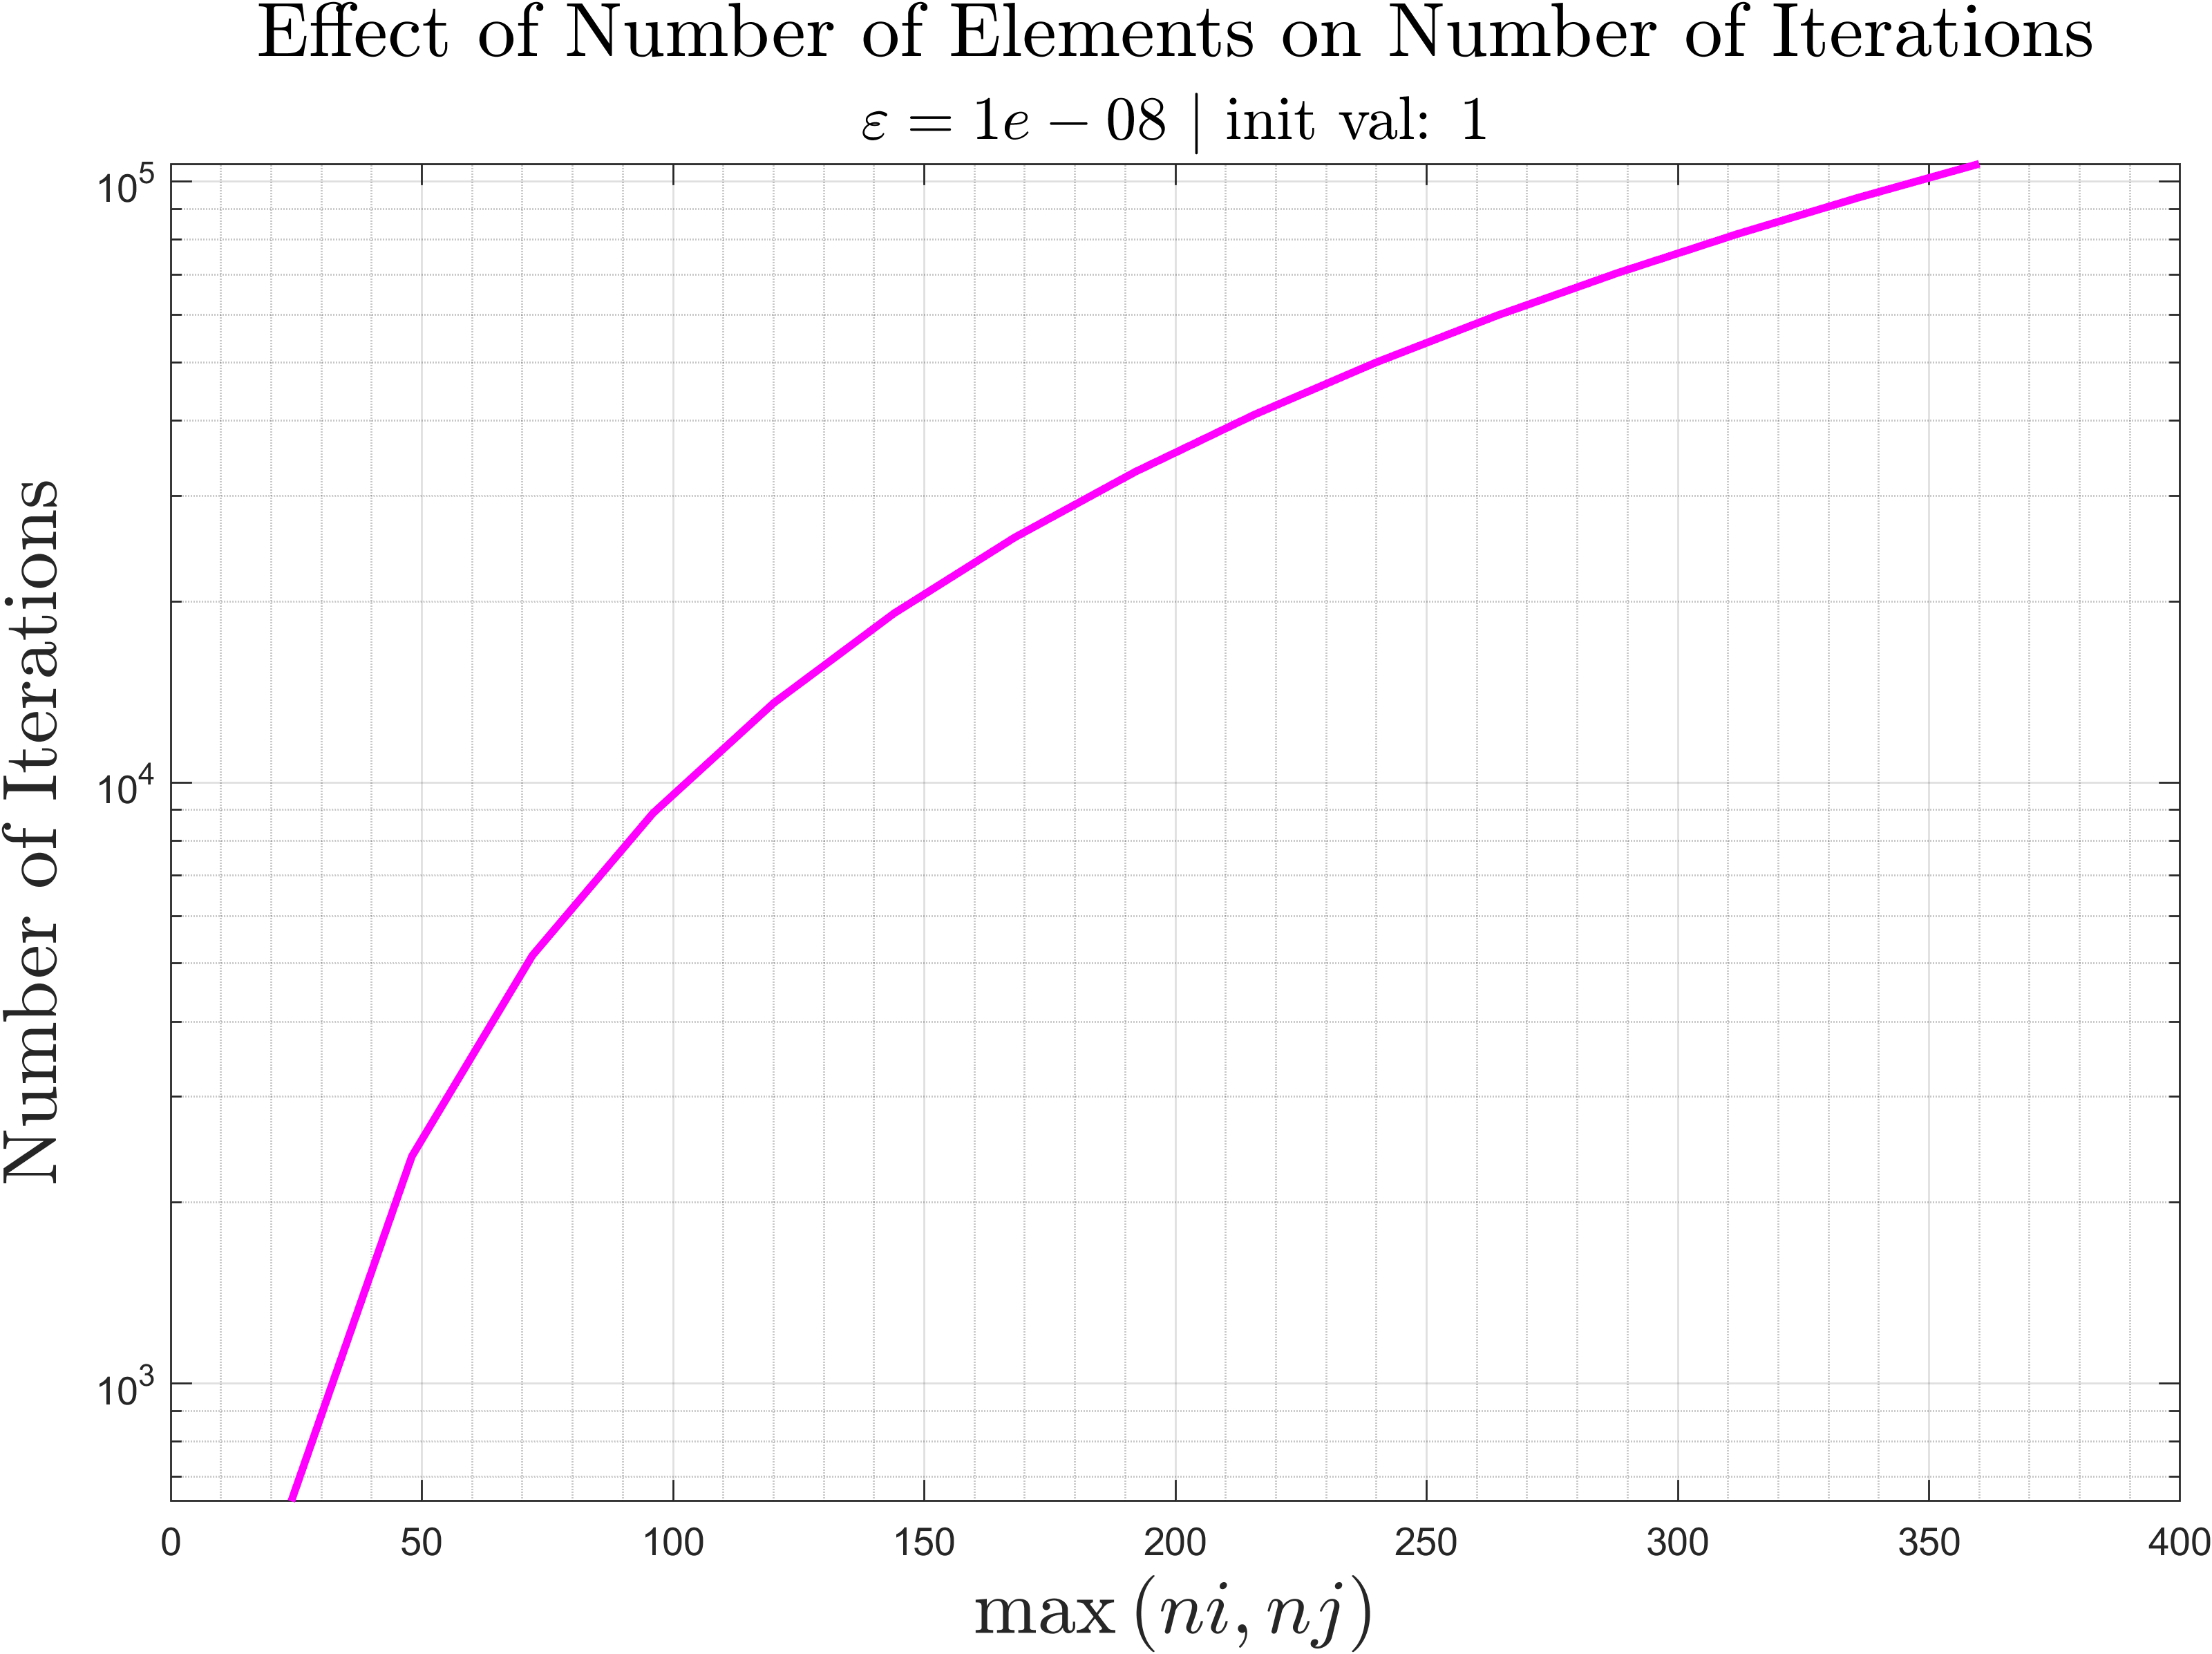
\includegraphics[width=\textwidth]{images/ni nj - n.png}
        \caption{Number of iterations as a function of maximum of ni and nj}
        \label{fig: n as a function of max ni nj}
    \end{subfigure}
    \hfill
    \begin{subfigure}[c]{0.49\textwidth}
        \centering
        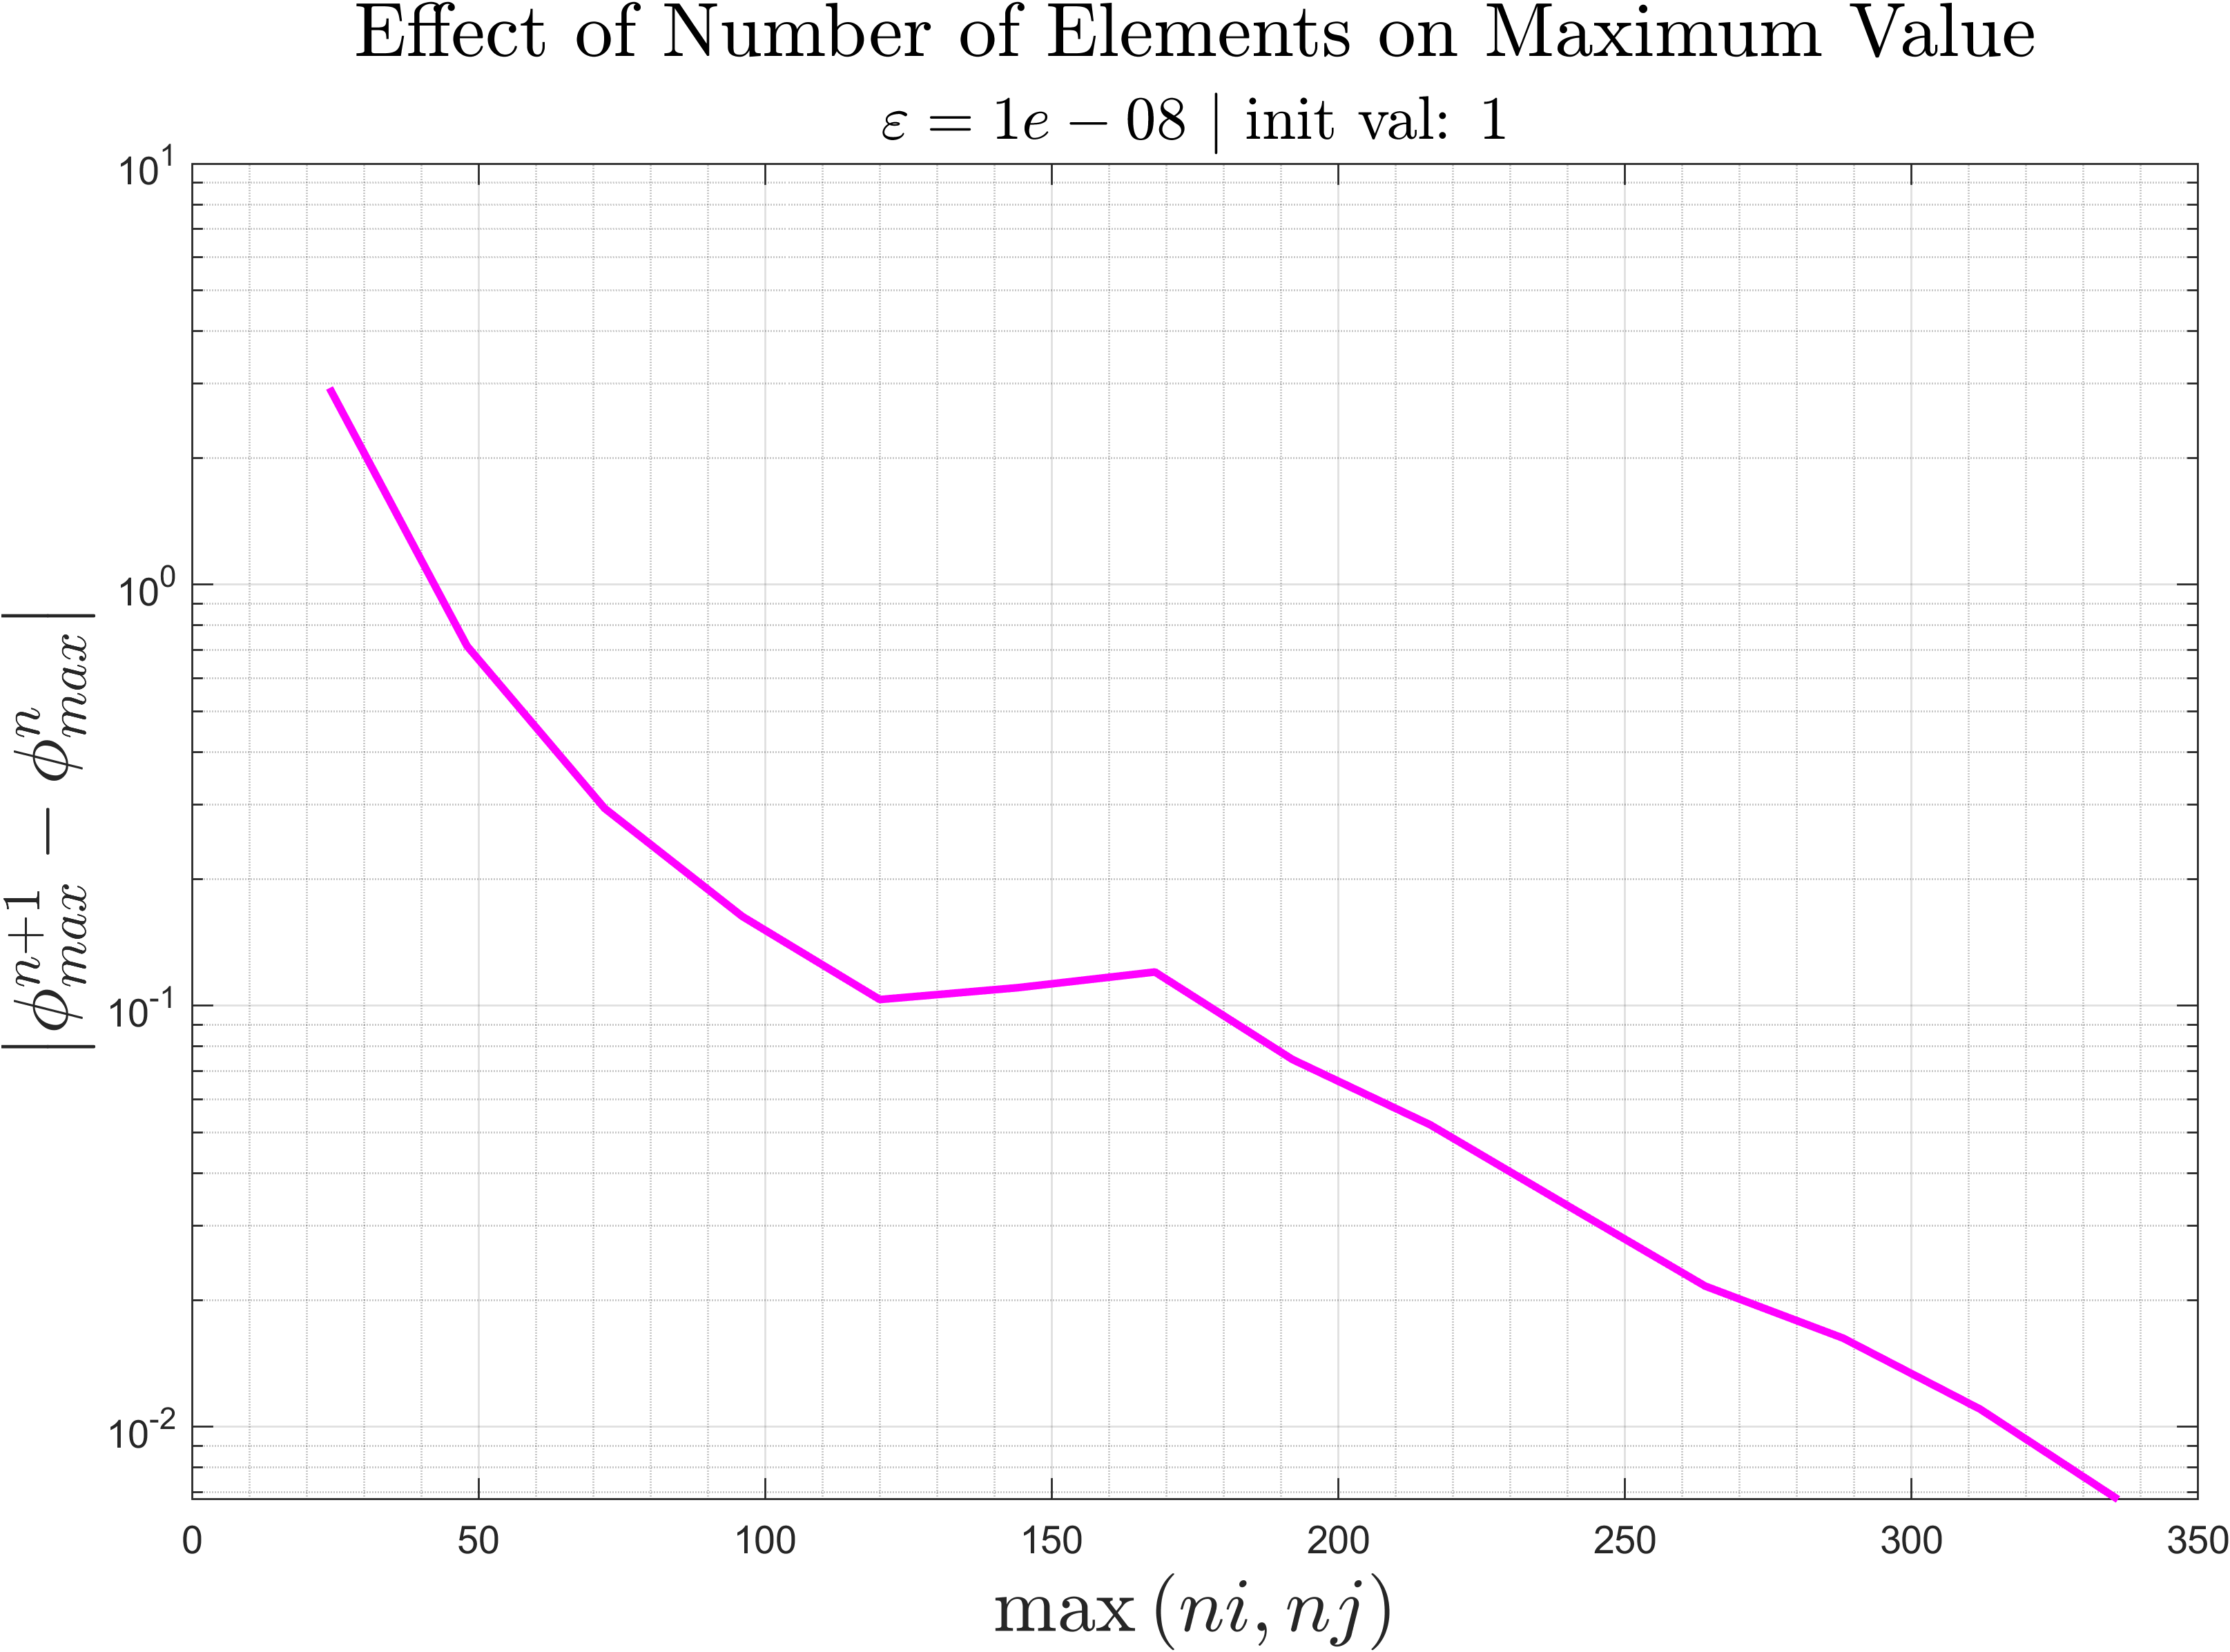
\includegraphics[width=\textwidth]{images/ni nj - max diff.png}
        \caption{Change in max value as a function of maximum of ni and nj}
        \label{fig: change in max value as a function of max ni nj}
    \end{subfigure}
    \caption{Influence of the number of elements ni nj}
    \label{fig: Influence of ni nj}
\end{figure}
We can see that as the number of grid points increases, the number of iterations increases and the error decreases. Since there is no clear optimal number of grid points we will choose a number that will have a sufficiently small error but not too much of iterations. Hence the chosen number of grid points will be 120.
\subsection{Influence of Convergence Criteria $\varepsilon$}
\begin{figure}[H]
    \centering
    \begin{subfigure}[c]{0.49\textwidth}
        \centering
        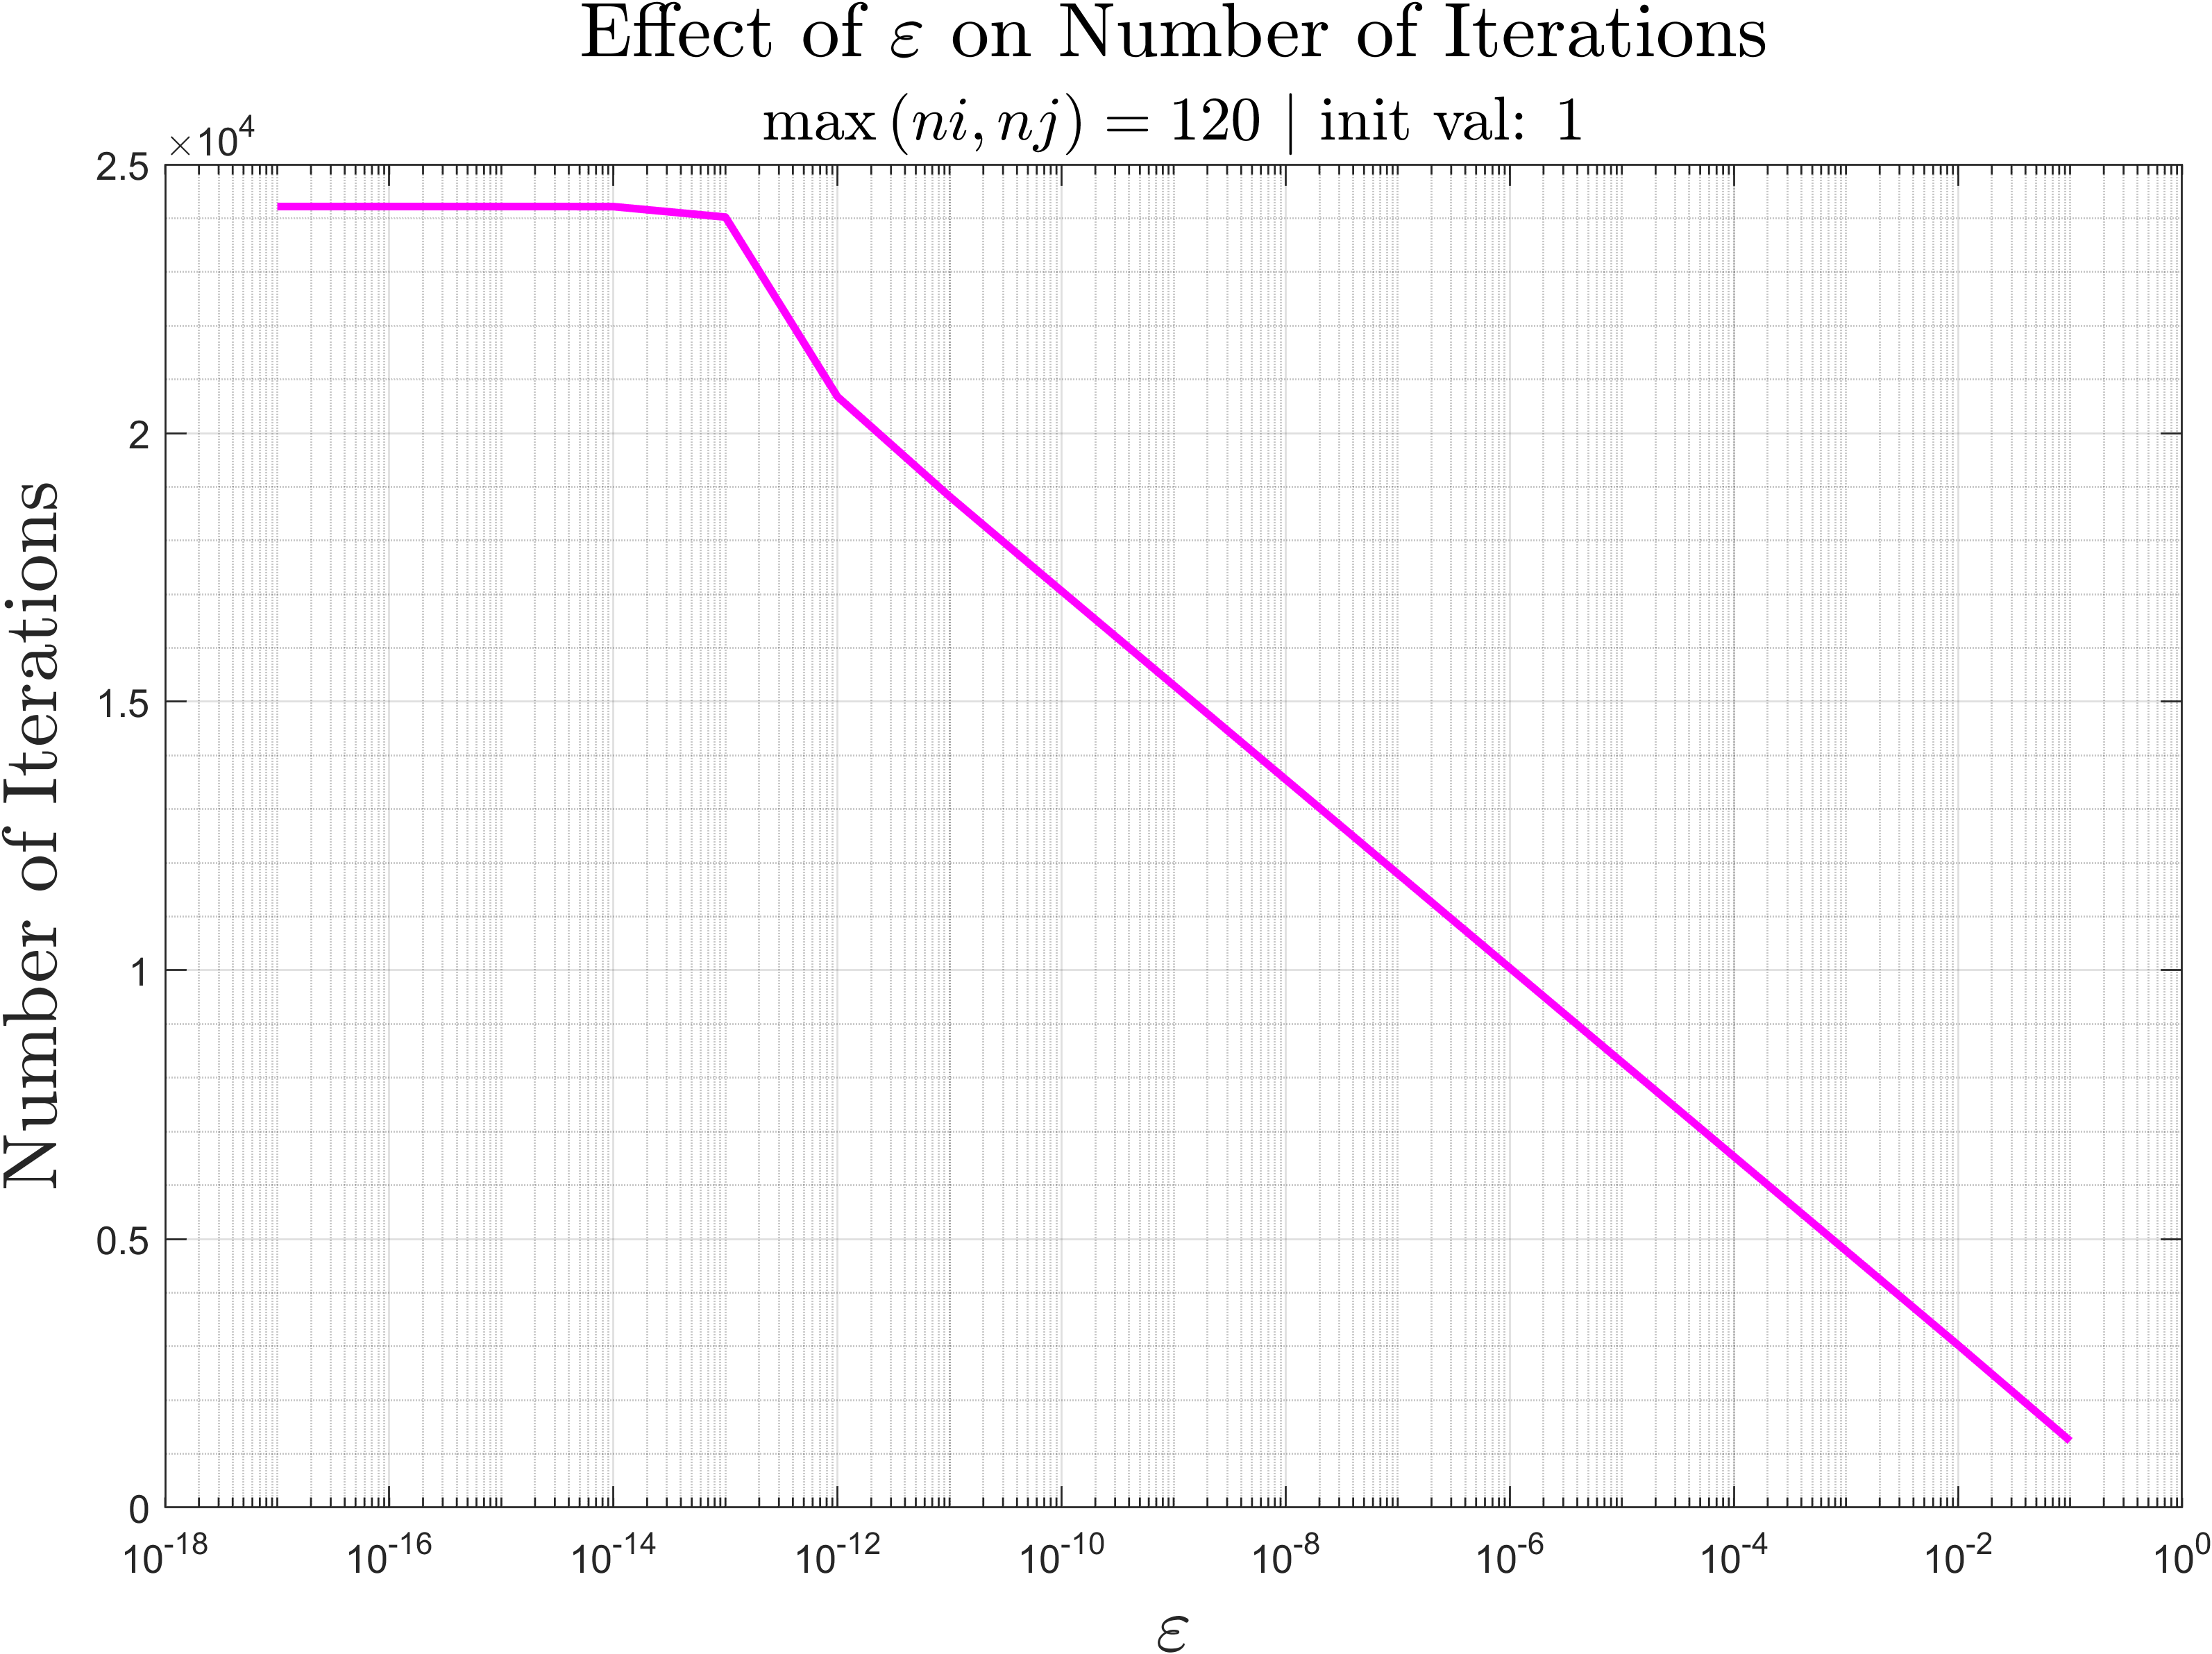
\includegraphics[width=\textwidth]{images/epsilon - n.png}
        \caption{Number of iterations as a function of $\varepsilon$}
        \label{fig: n as a function of epsilon}
    \end{subfigure}
    \hfill
    \begin{subfigure}[c]{0.49\textwidth}
        \centering
        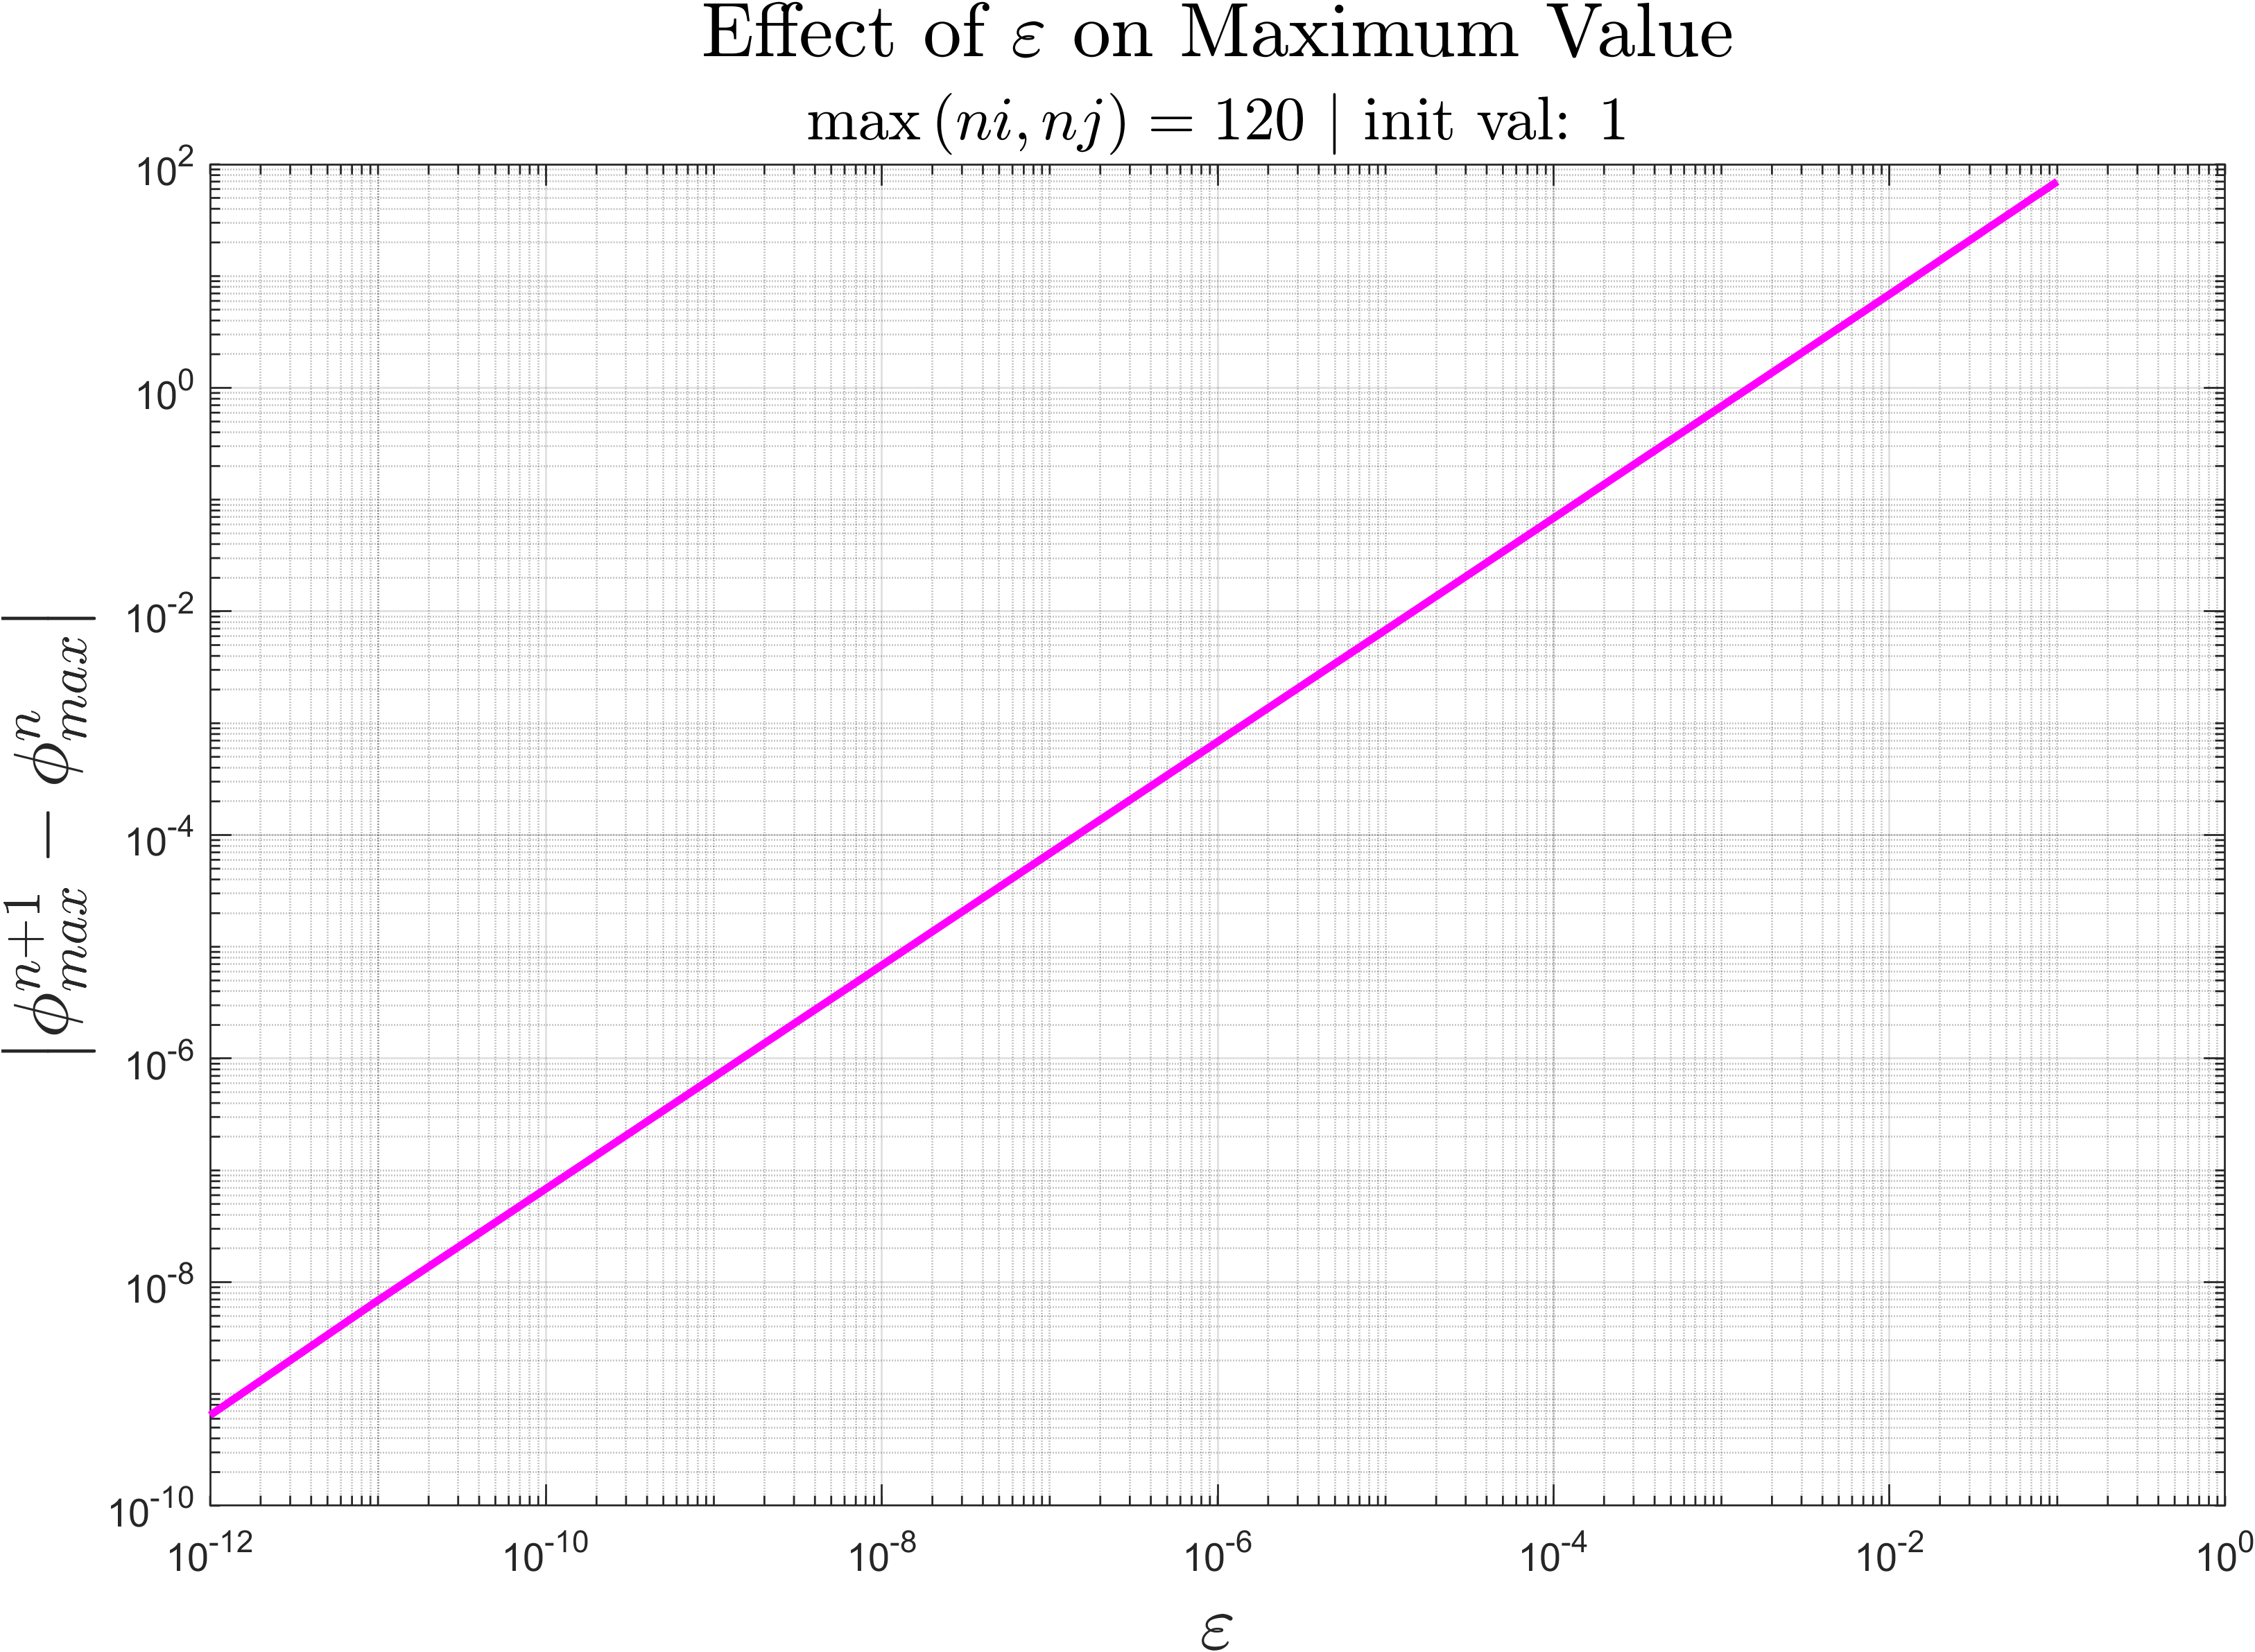
\includegraphics[width=\textwidth]{images/epsilon - max diff.png}
        \caption{Change in max value as a function of $\varepsilon$}
        \label{fig: change in max value as a function of epsilon}
    \end{subfigure}
    \caption{Influence of the convergence criteria $\varepsilon$}
    \label{fig: Influence of epsilon}
\end{figure}
Figure \ref{fig: Influence of epsilon} shows that as the convergence criteria decreases, the number of iterations increases up to a certain point. This point is probably the accuracy limitation of floating double point. Moreover, the error decreases exponentially with the decrease of the convergence criteria. We can declare that $\varepsilon=1\cdot10^{-8}$ is a good value for the convergence criteria.
\subsection{Influence of Initial Conditions}
\begin{figure}[H]
    \centering
    \begin{subfigure}[c]{0.49\textwidth}
        \centering
        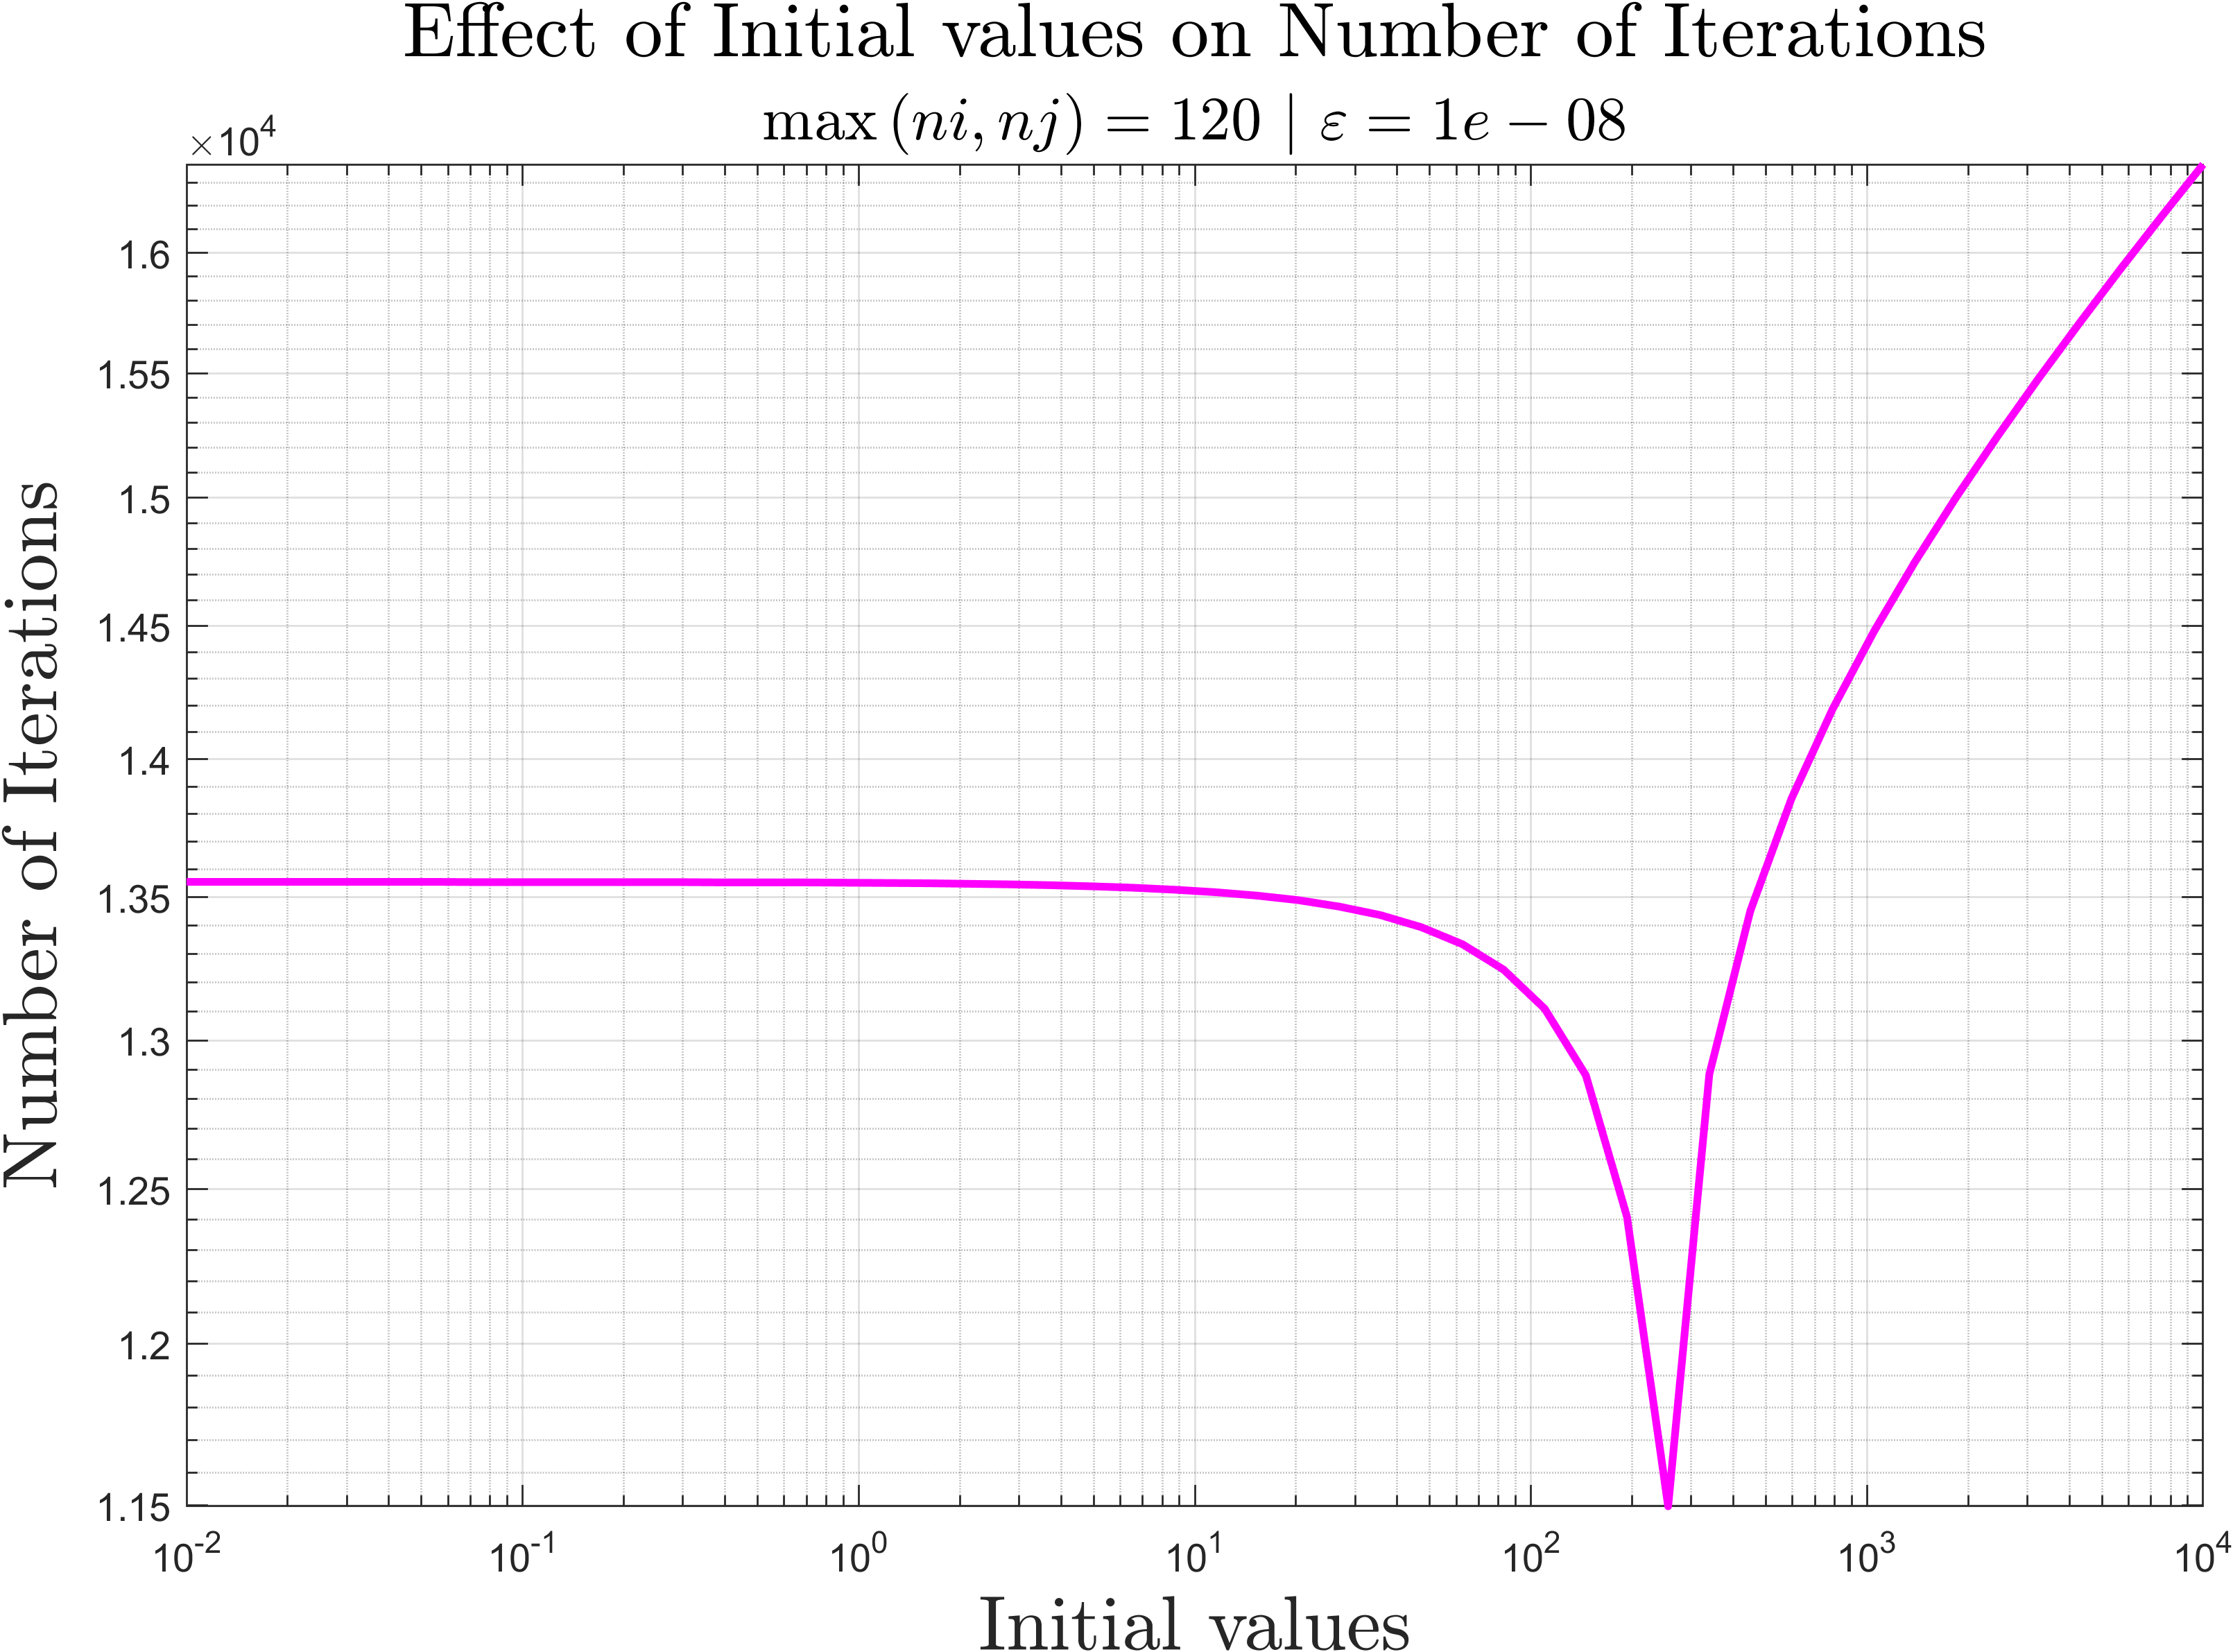
\includegraphics[width=\textwidth]{images/init val - n.png}
        \caption{Number of iterations as a function of initial value}
        \label{fig: n as a function of init val}
    \end{subfigure}
    \hfill
    \begin{subfigure}[c]{0.49\textwidth}
        \centering
        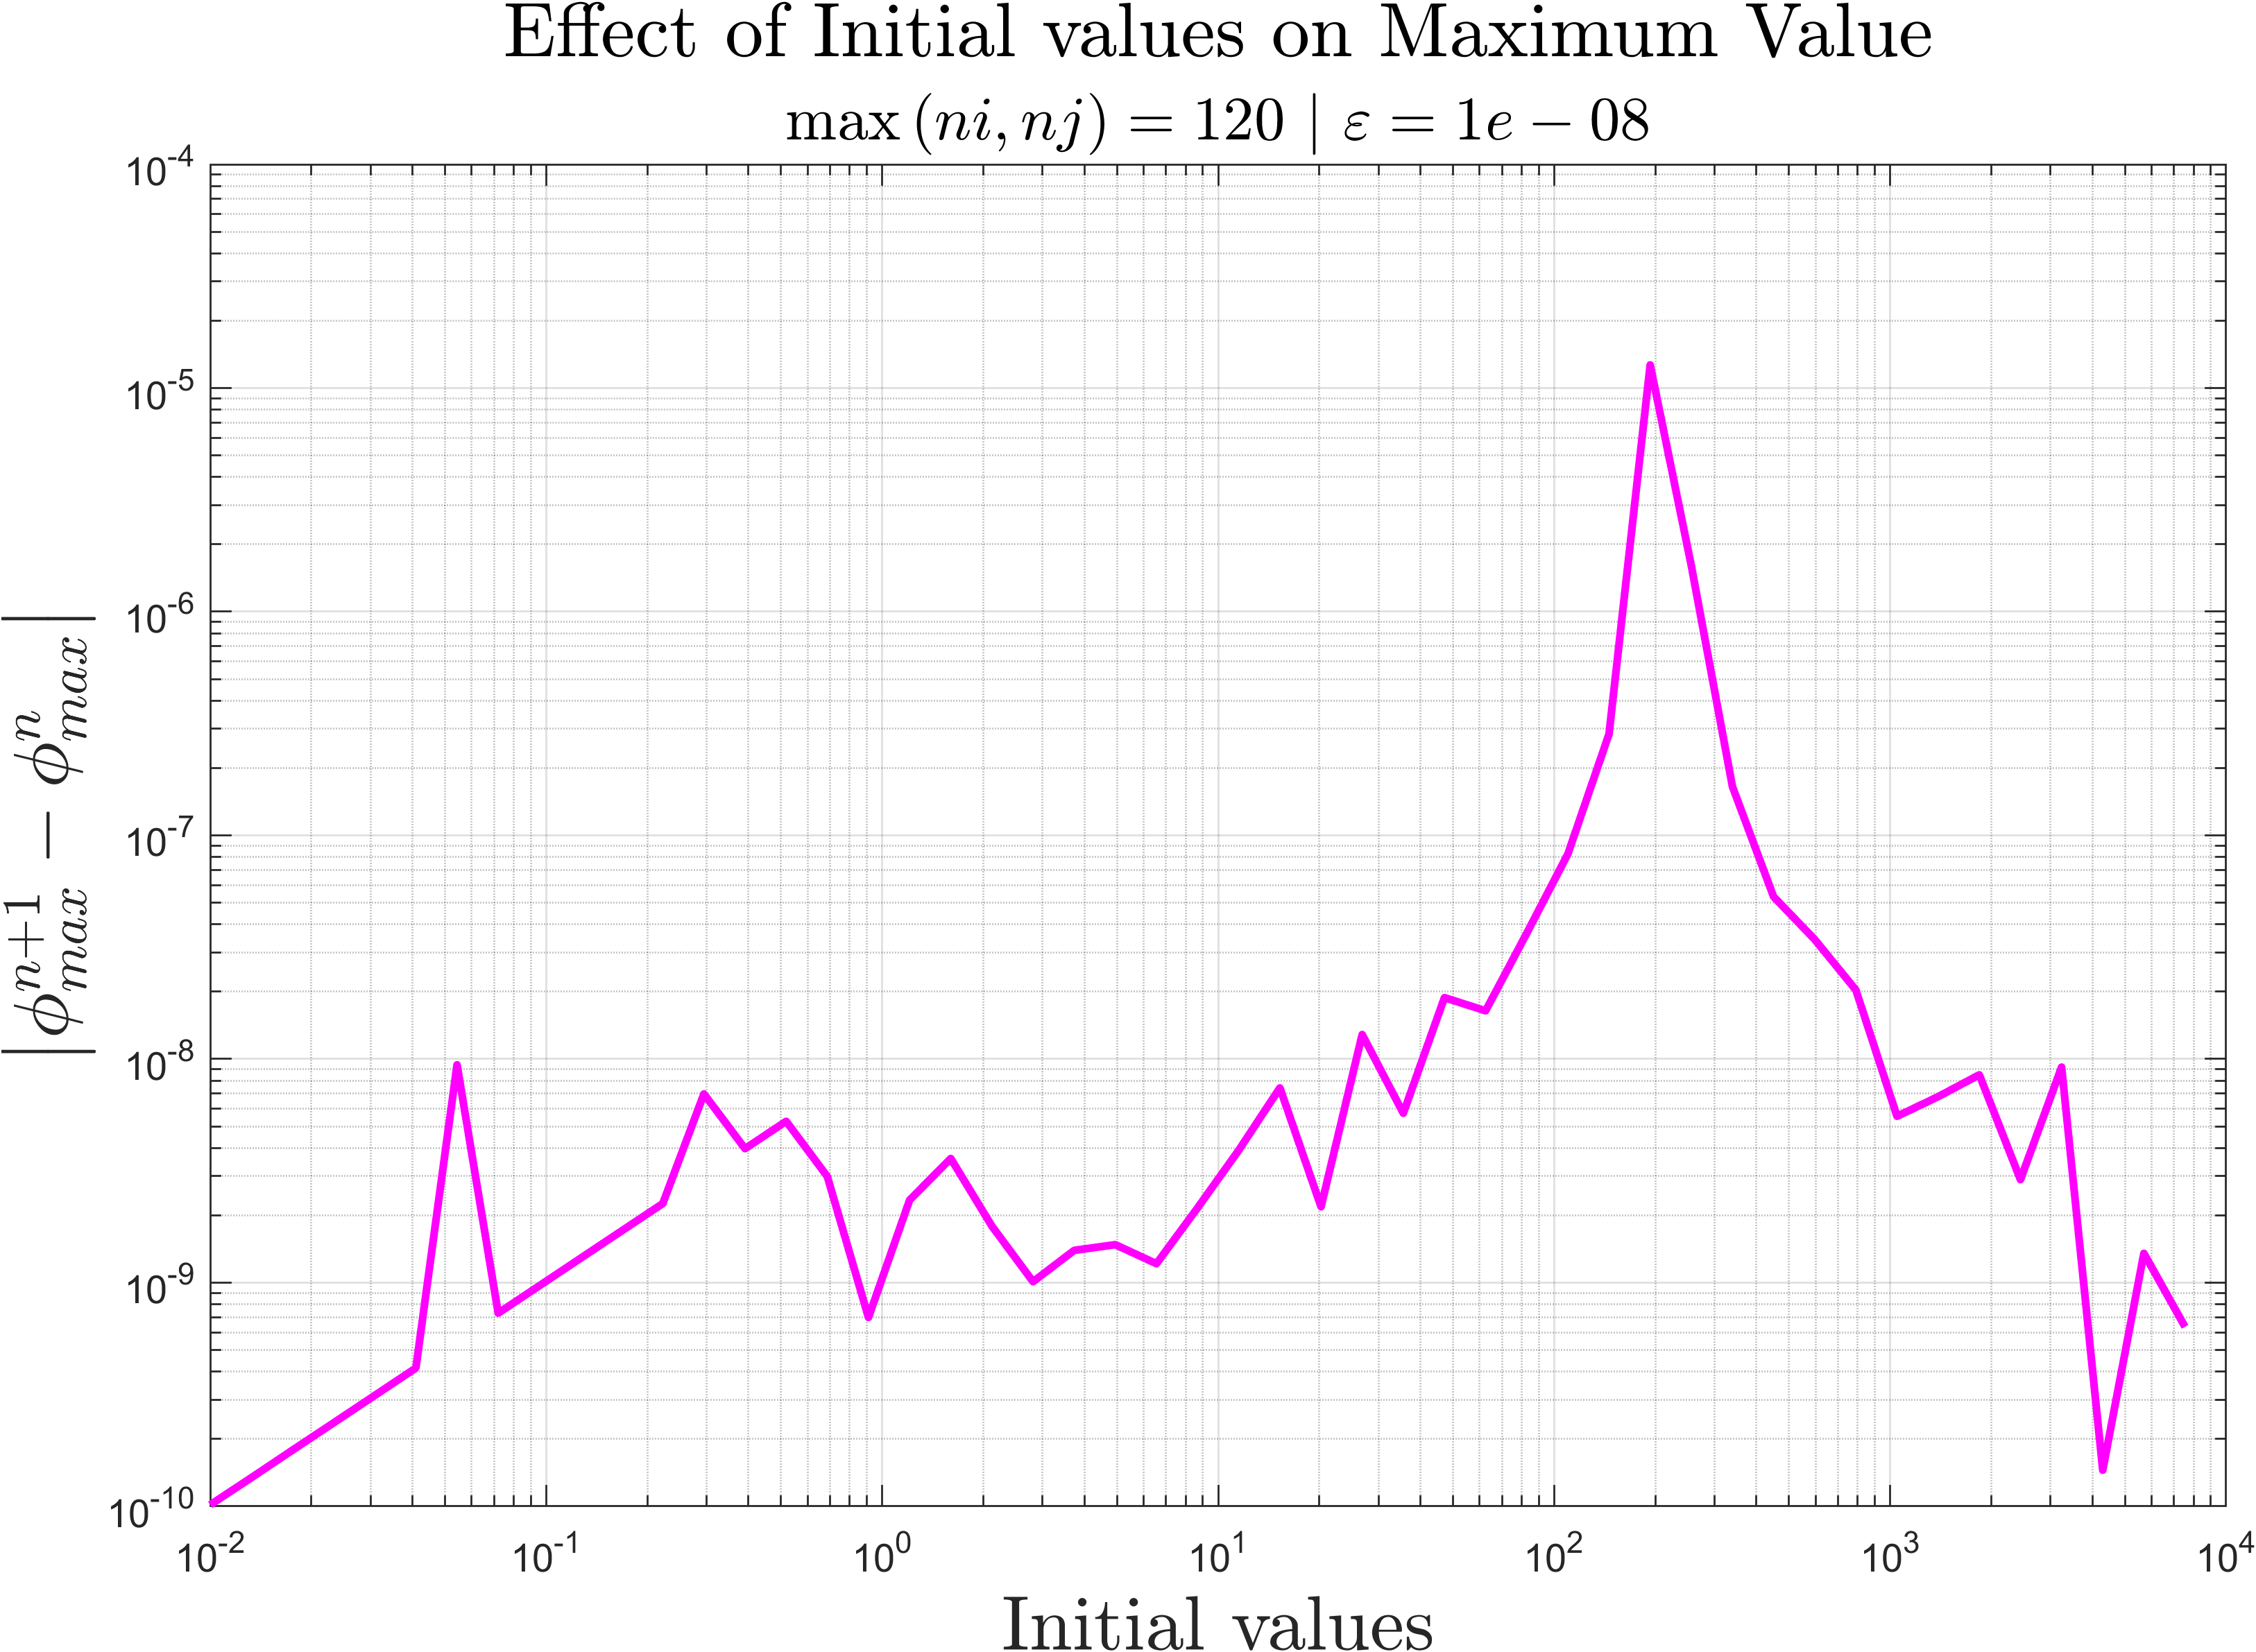
\includegraphics[width=\textwidth]{images/init val - max diff.png}
        \caption{Change in max value as a function of initial value}
        \label{fig: change in max value as a function of init val}
    \end{subfigure}
    \caption{Influence of the initial value}
    \label{fig: Influence of init val}
\end{figure}
We can see from Fig.\ref{fig: Influence of init val} that when the initial value is close the the maximal value of the flow, the number of iterations decreases but the error increases. Furthermore, for all initial values below 10, the number of iterations stays constant and the error has close to no change. So all initial values smaller than 10 are good and we will choose the initial value to be 1.

\section{Results and Discussion}
\label{sec: results and discussion}
\begin{figure}[H]
    \centering
    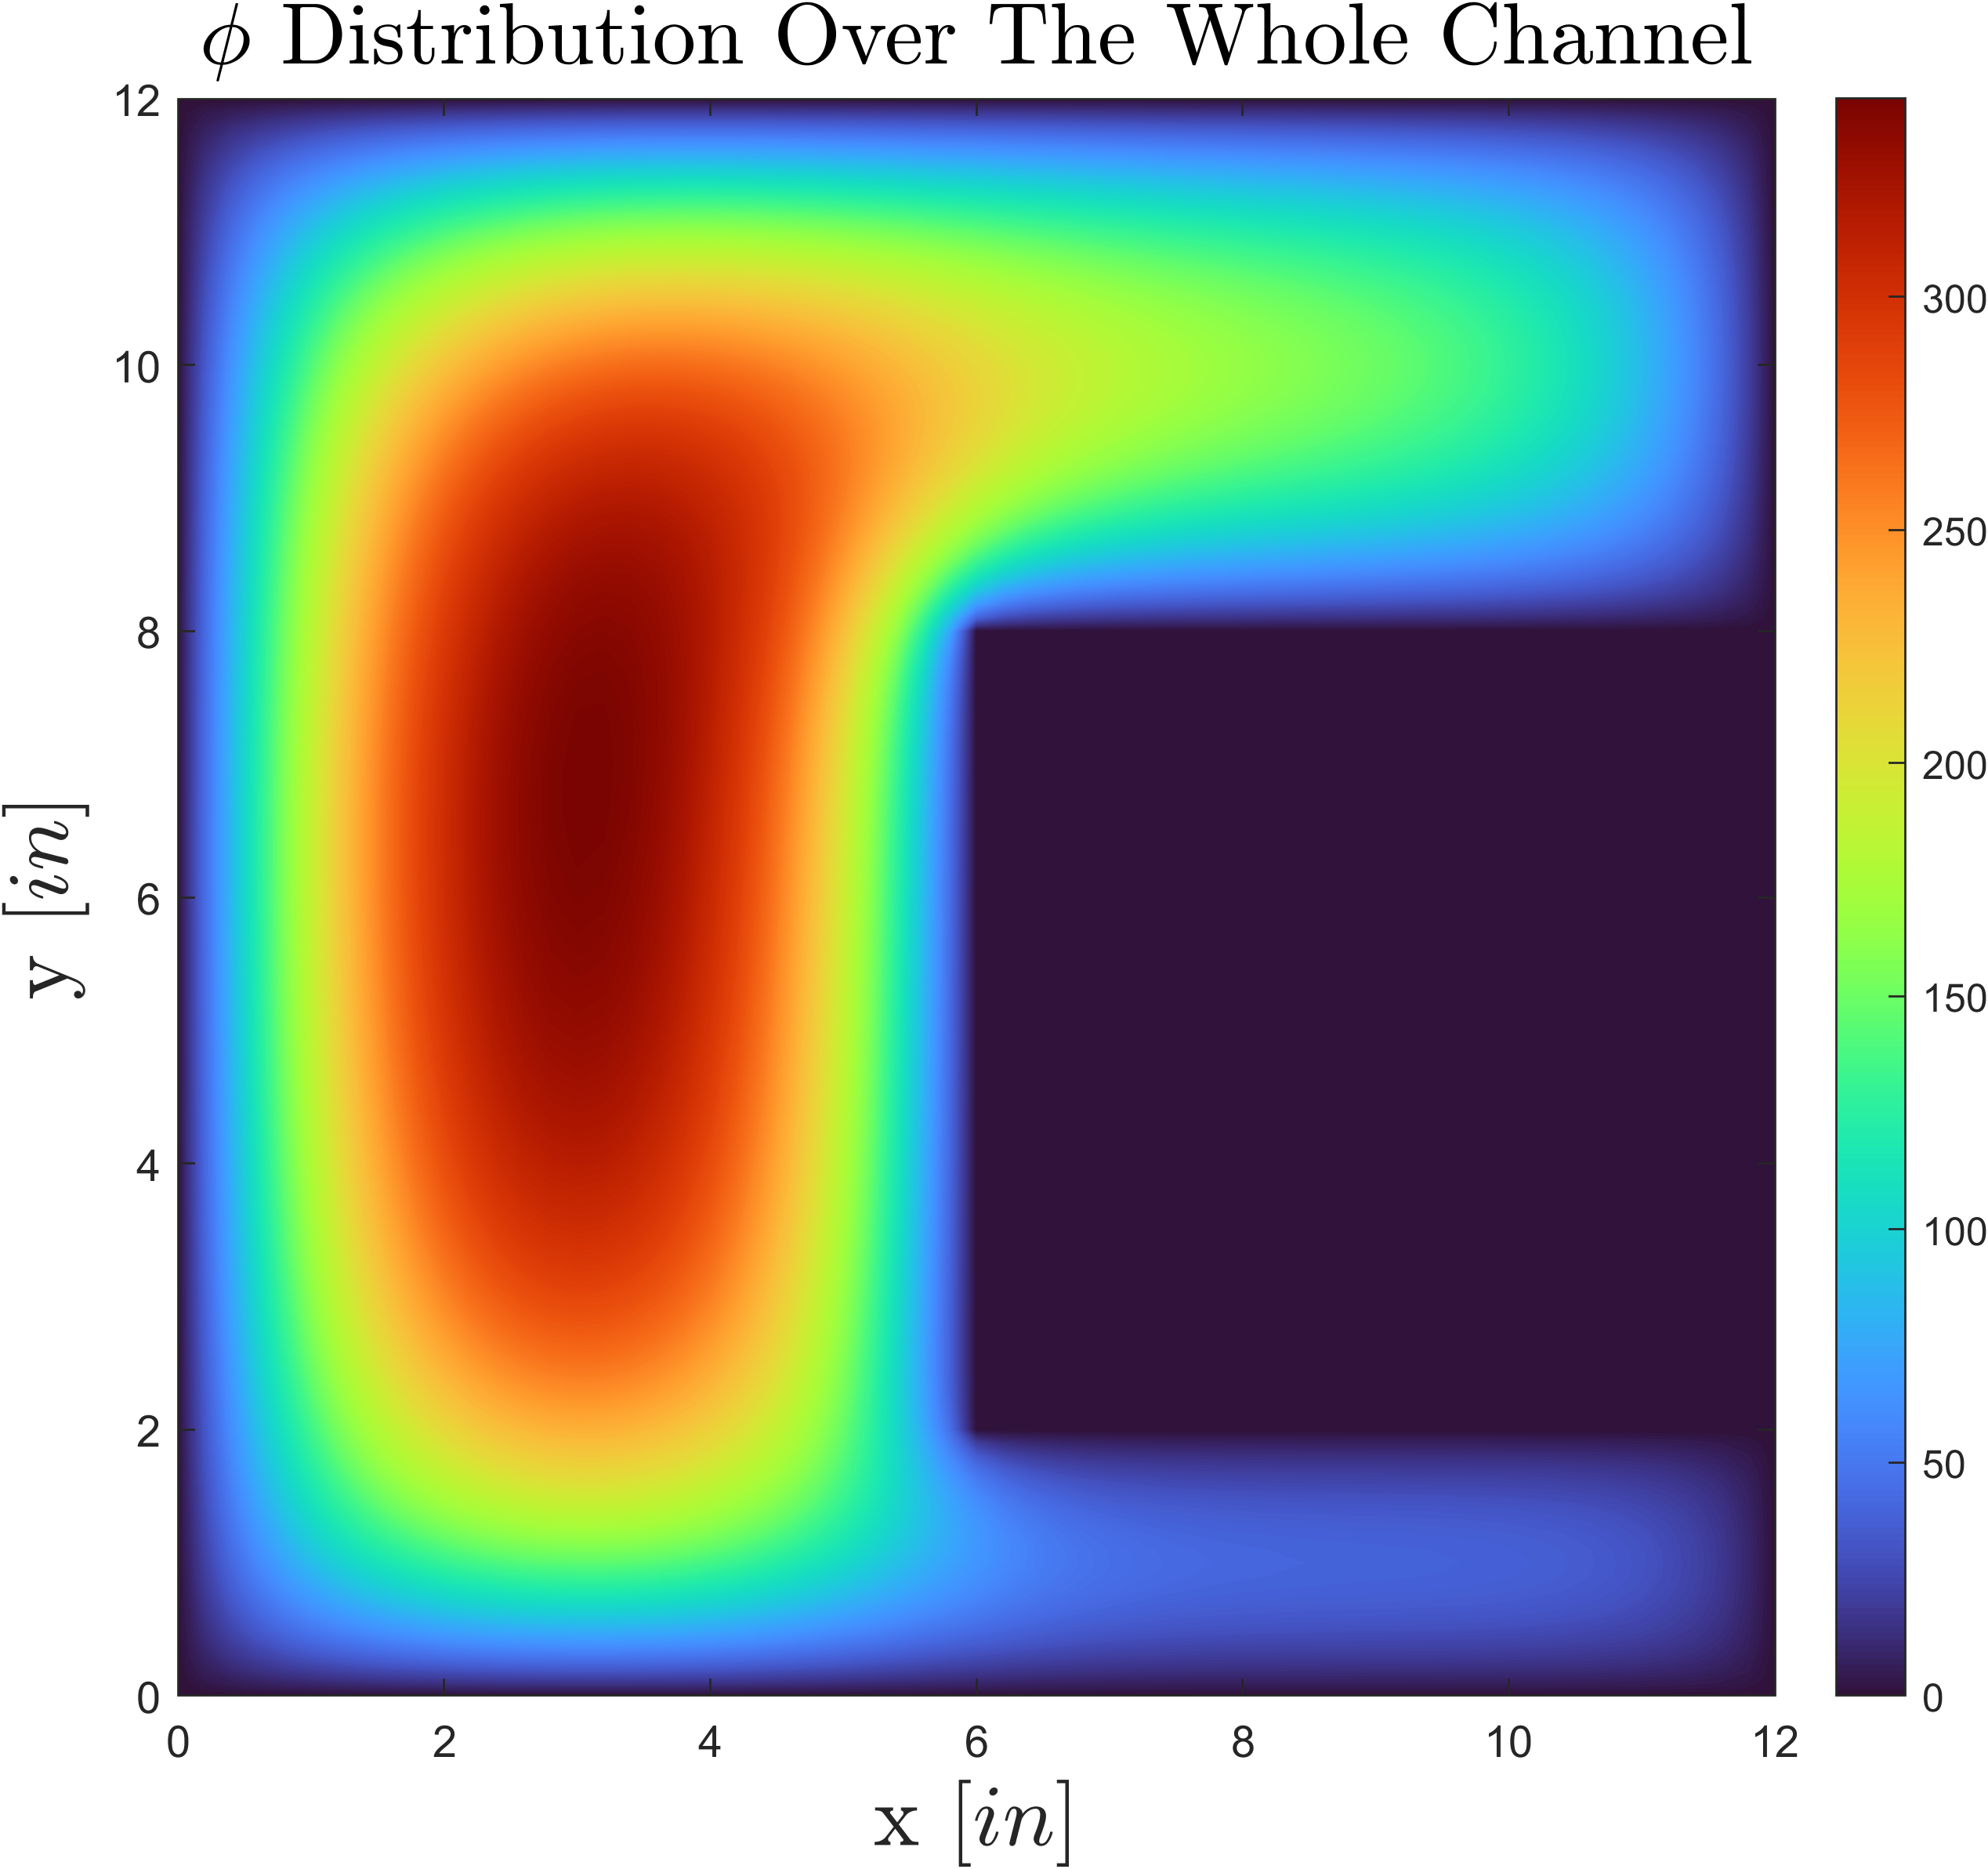
\includegraphics[width=0.6\textwidth]{images/phi ditribution.png}
    \caption{$\phi$ distribution over the whole field}
    \label{fig: phi distribution}
\end{figure}
We can see that as expected, the highest value of $\phi$ in the flow field is at the widest section of the channel. Moreover, this figure helps us to make sure that the no-slip and no-penetration conditions are enforced.

\section{Summary and Conclusion}

\newpage
\appendix
\section{Listing of The Computer Program}
\subsection{Parameters}
\begin{lstinputlisting}[captionpos=b,stringstyle=\color{magenta},frame=single, numbers=left, style=MatLab-editor, basicstyle=\mlttfamily\small, caption={Parameters file},mlshowsectionrules=true]{./matlab/parameters.m}
\end{lstinputlisting}
\begin{lstinputlisting}[captionpos=b,stringstyle=\color{magenta},frame=single, numbers=left, style=MatLab-editor, basicstyle=\mlttfamily\small, caption={Extra parameters file},mlshowsectionrules=true]{./matlab/calc_extra_param.m}
\end{lstinputlisting}

\subsection{Main Code}
\begin{lstinputlisting}[captionpos=b,stringstyle=\color{magenta},frame=single, numbers=left, style=MatLab-editor, basicstyle=\mlttfamily\small, caption={The main file},mlshowsectionrules=true]{./matlab/NM_hw3_CA.m}
\end{lstinputlisting}

\end{document}